\documentclass[]{article}
\usepackage{amsmath, amssymb, amsthm, graphicx}
\usepackage[shortlabels]{enumitem}

\DeclareMathOperator{\Hom}{Hom}
\DeclareMathOperator{\Det}{det}
\DeclareMathOperator{\supp}{supp}
\DeclareMathOperator{\id}{id}
\theoremstyle{definition}
\newtheorem{theorem}{Theorem}[section] % reset theorem numbering for each chapter

\theoremstyle{definition}
\newtheorem{definition}[theorem]{Definition} % definition numbers are dependent on theorem numbers

\newenvironment{sketch}{
	\renewcommand{\proofname}{Sketch of Proof}\proof}{\endproof}

\newtheorem{corollary}[theorem]{Corollary}
\newtheorem{lemma}[theorem]{Lemma}
\newtheorem{proposition}[theorem]{Proposition}
\begin{document}
\title{Differentiable Manifolds and the Hairy Ball Theorem}
\author{Jonathan Lau}
\maketitle

\section{Manifolds and Tangent Spaces}

\begin{definition}
    The upper half space is \[\mathcal{H}^n=\{(x_1, \dots, x_n)\in \mathbb{R}^n\mid x_n \geq 0\}.\] Its boundary is $\partial \mathcal{H}^n = \{(x_1, \dots, x_n)\in \mathbb{R}^n\mid x_n = 0\}$, and its interior is $\mathcal{H}^n \backslash \partial \mathcal{H}^n $.
\end{definition}

\begin{definition}[Smooth maps]
    Let $S$ be a subset of $\mathbb{R}^n$. A map $f:S \rightarrow \mathbb{R}^m$ is smooth at $p$ if there exists a neighborhood $U$ of $p$ and a smooth function $f':U \rightarrow \mathbb{R}^m$ such that $f'=f$ on $U\cap S$. If $f$ is smooth at every $p\in S$, then $f$ is smooth on $S$.
    In addition, if $F$ is bijective and $F^{-1}$ is smooth, then $F$ is called a diffeomorphism.
\end{definition}

Many properties of smooth maps on open sets also hold for smooth maps on arbitrary subsets. We will not prove them.

\begin{definition}
    Let $M$ be a Hausdorff, second countable topological space. A chart on $M$ is a pair $(U, \phi)$ where $U$ is open in $M$ and $\phi:U\rightarrow \mathcal{H}^n$ is a homeomorphism onto its image. Two charts $(U,\phi),(V,\psi)\in \mathcal{A}$ are compatible if the functions $\psi\circ\phi^{-1}$ and $\phi\circ\psi^{-1}$ are smooth on $\phi(U\cap V)$ and $\psi(U\cap V)$ respectively. An atlas $\mathcal{A}$ on $M$ is a collection of pairwise compatible charts that cover $M$.
\end{definition}


\begin{center}
    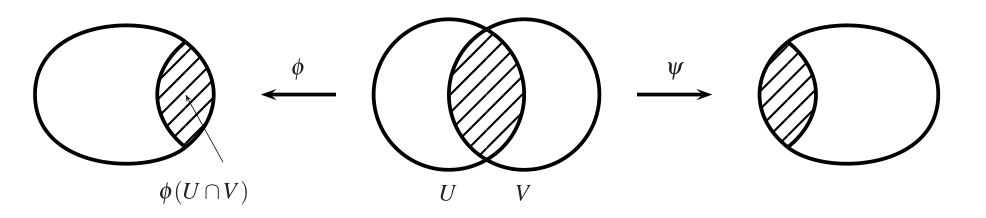
\includegraphics[scale=0.5]{compatible.png}
\end{center}

\begin{theorem}
    Each atlas is contained in a unique maximal atlas. That is, for each atlas $\mathcal{A}$ on $M$, there exists a unique atlas $\mathcal{U}$ on $M$ such that if $\mathcal{U}\subset\mathcal{U}'$, then $\mathcal{U}'=\mathcal{U}$.
\end{theorem}

\begin{proof}
    Let $\mathcal{A}$ be an atlas on $M$. Let $\mathcal{U}$ be the set of charts that are compatible with every chart in $\mathcal{A}$. Let $(U, \phi), (V, \psi)\in \mathcal{U}$, and let $p\in U\cap V$. There exists $(W, \sigma)\in \mathcal{A}$ such that $p\in W$. So, $\psi\circ\sigma^{-1}$ and $\sigma\circ\phi^{-1}$ are smooth at $\sigma(p)$ and $\phi(p)$ respectively. Therefore, \[\psi\circ\phi^{-1} = (\psi\circ\sigma^{-1})\circ(\sigma\circ\phi^{-1})\] is smooth at $\phi(p)$. As $p$ was arbitrary, $\psi\circ\phi^{-1}$ is smooth on $\phi(U\cap V)$. Similarly, $\phi\circ\psi^{-1}$ is smooth on $\psi(U\cap V)$, so $(U, \phi), (V, \psi)$ are compatible, and $\mathcal{U}$ is indeed an atlas.
    
    If $\mathcal{U}\subset \mathcal{U}'$, then every chart in $\mathcal{U}'$ is compatible with every chart in $\mathcal{U}$, in particular, with every chart in $\mathcal{A}$. By construction of $\mathcal{U}$, these charts are in $\mathcal{U}$, so $\mathcal{U}'\subset \mathcal{U}$, and $\mathcal{U}$ is maximal.

    Suppose $\mathcal{V}$ is a maximal atlas containing $\mathcal{A}$. Then, every chart in $\mathcal{V}$ is compatible with $\mathcal{A}$, so $\mathcal{V}\subset \mathcal{U}$. Similarly, $\mathcal{U}\subset \mathcal{V}$. This shows uniqueness, and concludes the proof.
\end{proof}

\begin{definition}
    A $n$ dimensional manifold with boundary $M$ is a Hausdorff, second countable topological space together with a maximal atlas.
\end{definition}

By Theorem 1.4, to construct a manifold, we only need to specify a topological space and an atlas. We write $M$ instead of $(M, \mathcal{A})$ for manifolds. From now on, when we say a chart on $M$, we mean a chart in $\mathcal{A}$.

\begin{theorem}[Smooth invariance of domain]
    Let $f:U\rightarrow S$ be a diffeomorphism, where $U$ is open in $\mathbb{R}^n$ and $S\subset \mathbb{R}^n$ is an arbitrary subset. Then $S$ is open in $\mathbb{R}^n$.
\end{theorem}
\begin{proof}
    Let $p\in U$. Since $f^{-1}$ is smooth, there exists a neighborhoog $V$ of $f(p)$ and a smooth function $g:V \rightarrow \mathbb{R}^n$ such that $g|_{V\cap S}=f^{-1}$. Then, $g\circ f$ is the identity on $f^{-1}(V)$, which is open. So, \[(Jg(f(p)))(Jf(p))=I\], and $\Det(Jf(p))\neq 0$. By the inverse function theorem, there are neighborhoods $U_p\subset U, V_{f(p)}\subset V$ such that $f:U_p \rightarrow V_{f(p)}$ is a diffeomorphism. We also have \[V_{f(p)}=f(U_p)\subset f(U)=S.\] For each $p\in U$, we can find an open set $V_{f(p)}\mathbb{R}^n$ such that $V_{f(p)}\subset S$. So, $S$ is open.
\end{proof}

\begin{corollary}
    Let $U$ and $V$ be open subsets of $\mathcal{H}^n$, and let $f:U \rightarrow V$ be a diffeomorphism. Then, $f$ maps interior points to interior points and boundary points to boundary points.
\end{corollary}
\begin{proof} 
    Suppose $p\subset U$ is an interior point. Then, it has an neighborhood $U_p$ open in $\mathbb{R}^n$. By the above theorem, $f(p)$ lies in the open set $f(U_p)$, so $f(p)$ is an interior point. Similarly, if $f(p)$ is an interior point, $f^{-1}(f(p))=p$ is an interior point.
\end{proof}

\begin{definition}
    Let $M$ be a manifold with boundary. A point $p$ is a boundary point if for some chart $(U, \phi)$, $\phi(p)\in \partial \mathcal{H}^n$. The set of all boundary points is the boundary $\partial M$.
\end{definition}

Suppose $(U,\phi),(V,\psi)$ are charts containing $p$, with $\phi(p)\in\partial \mathcal{H}^n $. By Corollary 1.7, $\psi(p)=\psi\circ\phi^{-1}(\phi(p))$ is also a boundary point, so boundary points are well defined.


\begin{definition}
    A manifold with boundary $M$ with empty boundary is called a manifold. For all charts $(U, \phi)$, the image of $\phi$ will be an open set in $\mathbb{R}^n$.
\end{definition}

\begin{proposition}
    Let $M$ be a manifold with non empty boundary. Then, $\partial M$ is a manifold.
\end{proposition}
\begin{proof}
    Let $\mathcal{A}$ be an atlas on $M$. For each $(U, \phi)\in \mathcal{A}$, we construct a chart $(U\cap \partial M , \phi|_{\partial M})$ on $\partial M$. These charts are compatible, and map into $\mathbb{R}^{n-1}$, so $\partial M$ is a manifold of dimension $n-1$.
\end{proof}

\begin{definition}[Smooth Functions]
    Let $N,M$ be manifolds. A continuous function $F:N\rightarrow M$ is smooth if for all charts $(U, \phi)$ on $N$ and $(V, \psi)$ on $M$, $\psi\circ F\circ \phi^{-1}$ is smooth. If $F$ is bijective and $F^{-1}$ is also smooth, then $F$ is a diffeomorphism.
\end{definition}

\begin{center}
    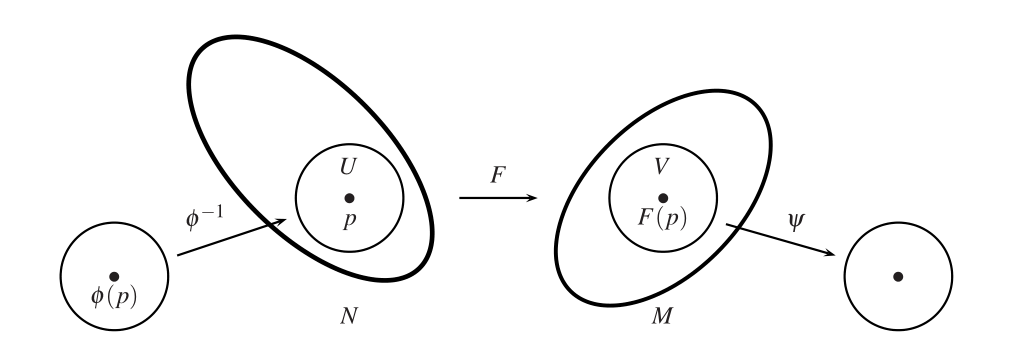
\includegraphics[scale=0.5]{smooth_function.PNG}
\end{center}

Unless stated otherwise, all functions are smooth.

\begin{definition}[Partial derivatives]
    Let $f:M \rightarrow \mathbb{R}$ and $(U, x_1, \dots, x_n)$ be a chart. The partial derivative of $f$ with respect to $x_i$ at $p$ is the derivative with respect to standard coordinates
    \[\frac{\partial}{\partial x_i}\bigg|_p f=\frac{\partial}{\partial r_i}\bigg|_{\phi(p)}(f\circ\phi^{-1}).\]
\end{definition}

\begin{definition}[Germs of functions]
    Let $M$ be a manifold, and $p\in M$. Let $S$ be the set of all smooth functions defined on a neighborhood of $p$. For $f, g\in S$, we define an equivalence relation by $f\sim g$ if there is a neighborhood of $p$ on which $f=g$. These equivalence classes are the germs of $M$ at $p$, denoted $C^\infty_p(M)$.
\end{definition}

\begin{definition}
    Let $M$ be a manifold, and $p\in M$. A derivation at $p$ is a linear map $D:C^\infty_p(M) \rightarrow \mathbb{R}$ such that $D(fg)=D(f)g(p)+f(p)D(g)$.
\end{definition}

\begin{definition}
    A tangent vector at $p$ is a derivation at $p$. The tangent space of $M$ at $p$ is the set of all derivations, denoted $T_pM$.
\end{definition}

$\frac{\partial}{\partial x_1}|_p, \dots, \frac{\partial}{\partial x_n}|_p$ are examples of tangent vectors. 

\begin{definition}
    Let $F: N \rightarrow M$ be a smooth function. We define the differential of $F$ to be a function\[F_*:T_pN \rightarrow T_{F(p)}M\] defined by \[F_*(X_p)(f)=X_p(f\circ F)\quad \text{ for } f\in C^\infty_{F(p)}(M).\]
\end{definition}

It is straightforward to check that $T_pM$ is a vector space, and that $F_*$ is a linear map.

\begin{theorem}[Chain rule]
    Let $F:N \rightarrow M$, $G:M \rightarrow P$, and $p\in N$. Then, $(G\circ F)_*=G_*\circ F_*$.
\end{theorem}
\begin{proof}
    Let $X_p\in T_pN$ and $f$ be a smooth function in a neighborhood of $G(F(p))$. Then \[(G\circ F)_*(X_p)f=X_p(f\circ G\circ F)=(F_*X_p)(f\circ G)=(G_*\circ F_*(X_p))f.\]
\end{proof}

\begin{theorem}
    Let $(U, x_1, \dots, x_n)$ be a chart. Then, \[\frac{\partial}{\partial x_1}\bigg|_p, \dots, \frac{\partial}{\partial x_n}\bigg|_p\] is a basis for $T_pM$.
\end{theorem}
\begin{proof}
    By the chain rule, $\id=(\phi^{-1}\circ\phi)_*=\phi^{-1}_*\circ \phi_*$, so $\phi_*$ is an isomorphism. We see that \[\phi_*\left(\frac{\partial}{\partial x_i}\bigg|_p\right)f=\frac{\partial}{\partial x_i}\bigg|_p(f\circ\phi)=\frac{\partial}{\partial r_i}\bigg|_{\phi(p)}(f\circ\phi\circ\phi^{-1})=\frac{\partial}{\partial r_i}|_{\phi(p)}f.\] It remains to show that $\frac{\partial}{\partial r_i}|_{\phi(p)}$ is a basis of $T_{\phi(p)}\mathbb{R}^n$. For simplification, we replace $\phi(p)$ by $p$.

    Suppose $\sum_{i=1}^{n}a_i\frac{\partial}{\partial r_i}|_{p}=0$. Applying to the coordinate functions $r_i$, we see that $a_i=0$.

    Next, we show that they span the space. Let $D$ be a derivation, and $f$ a smooth function. We technically require $f$ to be a germ, but the argument still holds. By Taylor's theorem, \[f(x)=f(p)+\sum_{i=1}^{n}(x_i-p_i)g_i(x)\quad g(p)=\frac{\partial f}{\partial x_i}(p).\] Using the Leibniz rule and linearity, \[Df(x)=\sum_{i=1}^{n}Dx_ig_i(p)=\sum_{i=1}^{n}Dx_i\frac{\partial}{\partial r_i}\bigg|_{p}f.\] We have cancelled the terms $Df(p)$ and $Dp_i$ since \[D(1)=D(1\cdot 1)=1D(1)+D(1)1=2D(1),\] so $D(1)=0$ and $D(c)=0$ by linearity. Thus, \[Df=\sum_{i=1}^{n}Dx_i\frac{\partial}{\partial r_i}\bigg|_{p}.\]
\end{proof}

\begin{definition}
    A $k$-form is a map that sends $p\in M$ to $\omega_p\in \Lambda^kT_pM$.
\end{definition}

We define $(dx_1)_p, \dots, (dx_n)_p$ to be the dual basis of $\frac{\partial}{\partial x_1}|_p, \dots, \frac{\partial}{\partial x_n}|_p$. By a result in multilinear algebra, $\{(dx_{i_1})_p\wedge\dots\wedge(dx_{i_k})_p\mid 1\leq i_1<\dots<i_n\leq n\}$ is a basis for $\Lambda^kT_pM$. If we fix a chart $(U, x_1, \dots, x_n)$, then we can write $\omega=\sum a_Idx_I$, where $a_I$ are real valued functions on $U$.

\begin{definition}
Let $\omega$ be a $k$-form. If for every chart $(U, x_1, \dots, x_n)$, the coefficients $a_I$ in $\omega=\sum a_Idx_I$ are smooth, then $\omega$ is smooth. The set of smooth $k$-forms is denoted $\Omega^k(M)$. The graded algebra $\bigoplus \Omega^k(M)$ is denoted $\Omega^*(M)$.
\end{definition}

\begin{definition}
    A vector field $X$ on $M$ is a function that assigns to each $p\in M$ a tangent vector $X_p\in T_pM$. A vector field is smooth if for every chart $(U, x_1, \dots, x_n)$, the coefficients $a_i$ in $X=\sum_{i=1}^na_i\frac{\partial}{\partial x_i}|_p$ are smooth. Given a 1-form $\omega$, we define $\omega(X):M \rightarrow \mathbb{R}, p\mapsto \omega_p(X_p)$.
\end{definition}

\begin{definition}
    An exterior derivative on $M$ is an $\mathbb{R}$-linear map $\Omega^*(M) \rightarrow \Omega^*(M)$ such that \begin{enumerate}
        \item $D(\omega\cdot \tau)=(D\omega)\cdot \tau+(-1)^k\omega\cdot D\tau$ for $\omega\in \Omega^k(M)$, $\tau\in \Omega^\ell(M)$,
        \item $D\omega\in\Omega^{k+1}(M)$ for $\omega\in\Omega^k(M)$,
        \item $D\circ D=0$,
        \item if $f:M \rightarrow \mathbb{R}$ is smooth and $X$ is a smooth vector field, then $(Df)X=Xf$.
    \end{enumerate}
\end{definition}

\begin{theorem}
    Let $(U, x_1, \dots, x_n)$ be a chart containing $p$. We define an operator $d_U:\Omega^*(U) \rightarrow \Omega^*(U)$ by \[d_Uf=\sum_{i=1}^n \frac{\partial f}{\partial x_i}dx_i,\ d_U\omega=\sum_I d_Uf\wedge dx_I,\text{ where }\omega=\sum_I f_I dx_I.\] Next, we define an operator $d:\Omega^*(M)\rightarrow \Omega^*(M)$ given by $(d\omega)_p=(d_U\omega)_p$ for some chart $(U, \phi)$ containing $p$. Then, $d$ is well defined, and it is the unique exterior derivative on $M$.
\end{theorem}
\begin{proof}
    See [Tu, Theorem 19.4, p.214].
\end{proof}

\begin{definition}[Pullback]
    Let $\omega_p\in \Lambda^kT_pM$ and $F:N \rightarrow  M$. The pullback of $\omega_p$ by $F$ is $F^*(\omega_p)\in \Lambda^kT_pN$, defined as \[F^*(\omega_p)(v_1,\dots,v_k)=\omega_p(F_*(v_1),\dots, F_*(v_k)).\]
    The pullback of a differential form $\omega$ is defined as $(F^*\omega)_p=F^*(\omega_p)$.
\end{definition}

\begin{proposition}
    $F^*d\omega=dF^*\omega$
\end{proposition}

\begin{proposition}
    If $\omega\in \Omega^k(M)$, then $F^*\omega\in \Omega^k(N)$.
\end{proposition}

\section{Integration of Differential $n$-Forms}

\begin{definition}
    An orientation on a manifold with boundary is a non-vanishing differential $n$-form.
\end{definition}

\begin{definition}
    An oriented atlas is an atlas $\mathcal{A}$ such that for all $(U, \phi),(V, \psi)\in \mathcal{A}$, $\Det(J(\psi\circ\phi ^{-1}))>0$.
\end{definition}

\begin{theorem}
    \[\text{Orientations} \iff \text{Oriented atlas}\]
    \[ \omega \iff \omega_p(e_1,\dots,e_n)>0,\] where $e_1,\dots,e_n$ is the basis induced by $(U, \phi)$.
\end{theorem}

\begin{definition}[Integration on a $\mathbb{R}^n$]
    Let $\omega$ be a $n$-form on $(U, \phi)$, where $U\subset\mathbb{R}^n$. Then $\omega=f(x)dx_1\wedge\dots\wedge dx_n$ for some smooth $f$. The integral of $\omega$ over $U$ is $\int_U\omega=\int_U f$.
\end{definition}

\begin{definition}[Integration on a chart]
    Let $\omega$ be a $n$-form on $(U, \phi)$. The integral of $\omega$ over $U$ is $\int_U\omega=\int_{\phi^{-1}(U)}(\phi^{-1})^*\omega$. 
\end{definition}

\begin{definition}[Partition of Unity]
    A partition of Unity on a manifold $M$ is a collection of nonnegative smooth functions $\{\rho_\alpha:M \rightarrow \mathbb{R}\}_{\alpha\in A}$ such that
    \begin{enumerate}[(i)]
        \item the collection of supports, $\{\supp\rho_\alpha\}_{\alpha\in A}$, is locally finite,
        \item $\sum_{\alpha\in A} \rho_\alpha = 1.$
    \end{enumerate}
\end{definition}

\begin{definition}[Integration on a Manifold]
    Let $\omega$ be a $n$-form on $M$. The integral of $\omega$ over $M$, denoted by $\int_M \omega$, is defined to be $\sum_{\alpha\in A}\int_{U_\alpha}\rho_\alpha\omega$.
\end{definition}

\begin{theorem}
    Let $\omega$ be a smooth $(n-1)$-form on $\mathcal{H}^n$ with compact support. Then $\int_{\mathcal{H}^n}d\omega=\int_{\partial \mathcal{H}^n}\omega$.
\end{theorem}

\begin{theorem}
    Let $\omega$ be a smooth $(n-1)$-form on an oriented manifold with boundary $M$. Then $\int_{M}d\omega=\int_{\partial M}\omega$.
\end{theorem}



\end{document}